\section{测试与结果}

前端使用 webpack 打包工具开发,运行在 9020 端口,而服务器使用 Node.js 开发,运行在 8600 端口,因为端口不同,浏览器的同源策略很阻止客户端和服务器的通信,需要配置代理,将 9020 端口数据转发到 8600 端口。同时为了使用 WebSocket 通信,服务器要配置启用 WebSocket 服务,访问地址不再是 http/https,而是 ws/wss。
在浏览器/服务器模式下使用 Websocket 模拟 1-RTT 握手 和 0-RTT 握手,打开网页首先进行 1-RTT 握手,客户端生成 32字节的随机数、32字节密钥,使用 x25519 曲线计算公钥,在 ClientHello 中发送给服务器,服务器收到 ClientHello 后也生成32字节随机数、32字节私钥,同样使用 x25519 曲线计算公钥,并且使用客户端的公钥计算共享密钥,最后发送 ServerHello 给客户端。

客户端和服务器通过计算椭圆曲线私钥和公钥。完成协商参数和计算后使用 HKDF 计算导出密钥,计算 Ticker 和 Binder。客户端使用 0-RTT 握手时,使用对应的密钥加密 Early Data 并发送给服务器。服务器读取文件系统中的证书和证明密钥,证书通过 Certificate 消息发送给客户端,然后使用导出密钥计算 Certificate Verify 发送到客户端,最后使用私钥签署整个握手过程,发送 Finished 消息。客户端通过导出密钥计算 Finished 消息发送到服务器,到此完成密钥交换、服务器参数和认证。

服务器接收到客户端的 Finished 消息后,可以马上发送两次 NewSessionTicker 消息,用于之后的 0-RTT 握手。测试 0-RTT 时候,首先断开第一次的 WebSocket 连接,再次打开浏览器,使用 WebSocket 连接的时候,客户端首先检查缓存中是否有对应域名的 Ticket,如果有就从浏览器的 Localstorage 中读取对应的 Ticket,使用之前保存下来的复用密钥加密早期数据,连同 ClientHello 一起发送给服务器,服务器检查 Ticket,判断 Ticket 的有效性,选择接受早期数据还是拒绝早期数据。收到服务器 Finished 消息的客户端还需要发送 EndOfEarlyData 消息表明自己早期数据发送完成。

在客户端和服务器端使用 JavaScript 的 Buffer 操作,使用 WebSocket 发送消息时候,需要发送文本信息。为了方便观察,把参数、证书、导出密钥等显示在浏览器上。 测试数据 Redis 初始化一万条数据量,使用 Node.js 作为后台服务器,测试抗重放功能。为此开发了具备功能齐全的后端服务器,比如注册、登陆、获取个人信息,获取最新新闻列表、转账等后台接口。

分别开发各种防御措施的中间件:1. 检查 Ticker 是否过期。2. 检查 Ticker 是否被使用。3. 控制器判断请求是否带有 Early Data 的请求头,进一步判断是否为幂等性的请求。首先用户登录会在服务器生成 PSK 的 Ticker 和 Binder,其中 Ticker 有效期具体设置为 5 分钟,然后保存到数据库。测试在 Ticker 有效期内的重放攻击。使用中间件判断 Ticker,可以更灵活,重用性高。

对于 Ticker 有效期内的正常 0-RTT,验证通过后使用 HKDF 从 PSK 中导出密钥,解密 Early Data。服务器接收到过期的 Ticker 或者重放攻击的 Ticker,都会被拒绝,编写重放攻击程序,并发数量为10个,持续重放 60 秒。结果见图1。 添加的 0-RTT 请求头,后台接口可以这个请求头灵活判断怎么应答 0-RTT 消息。比如根据分时间段出来 0-RTT,多数攻击者活动在晚上,在早上或者服务器高访问量的时候允许通过 0-RTT,到了晚上服务器访问量少的时候可以拒绝 0-RTT。

\begin{figure}[ht]
	\centering
	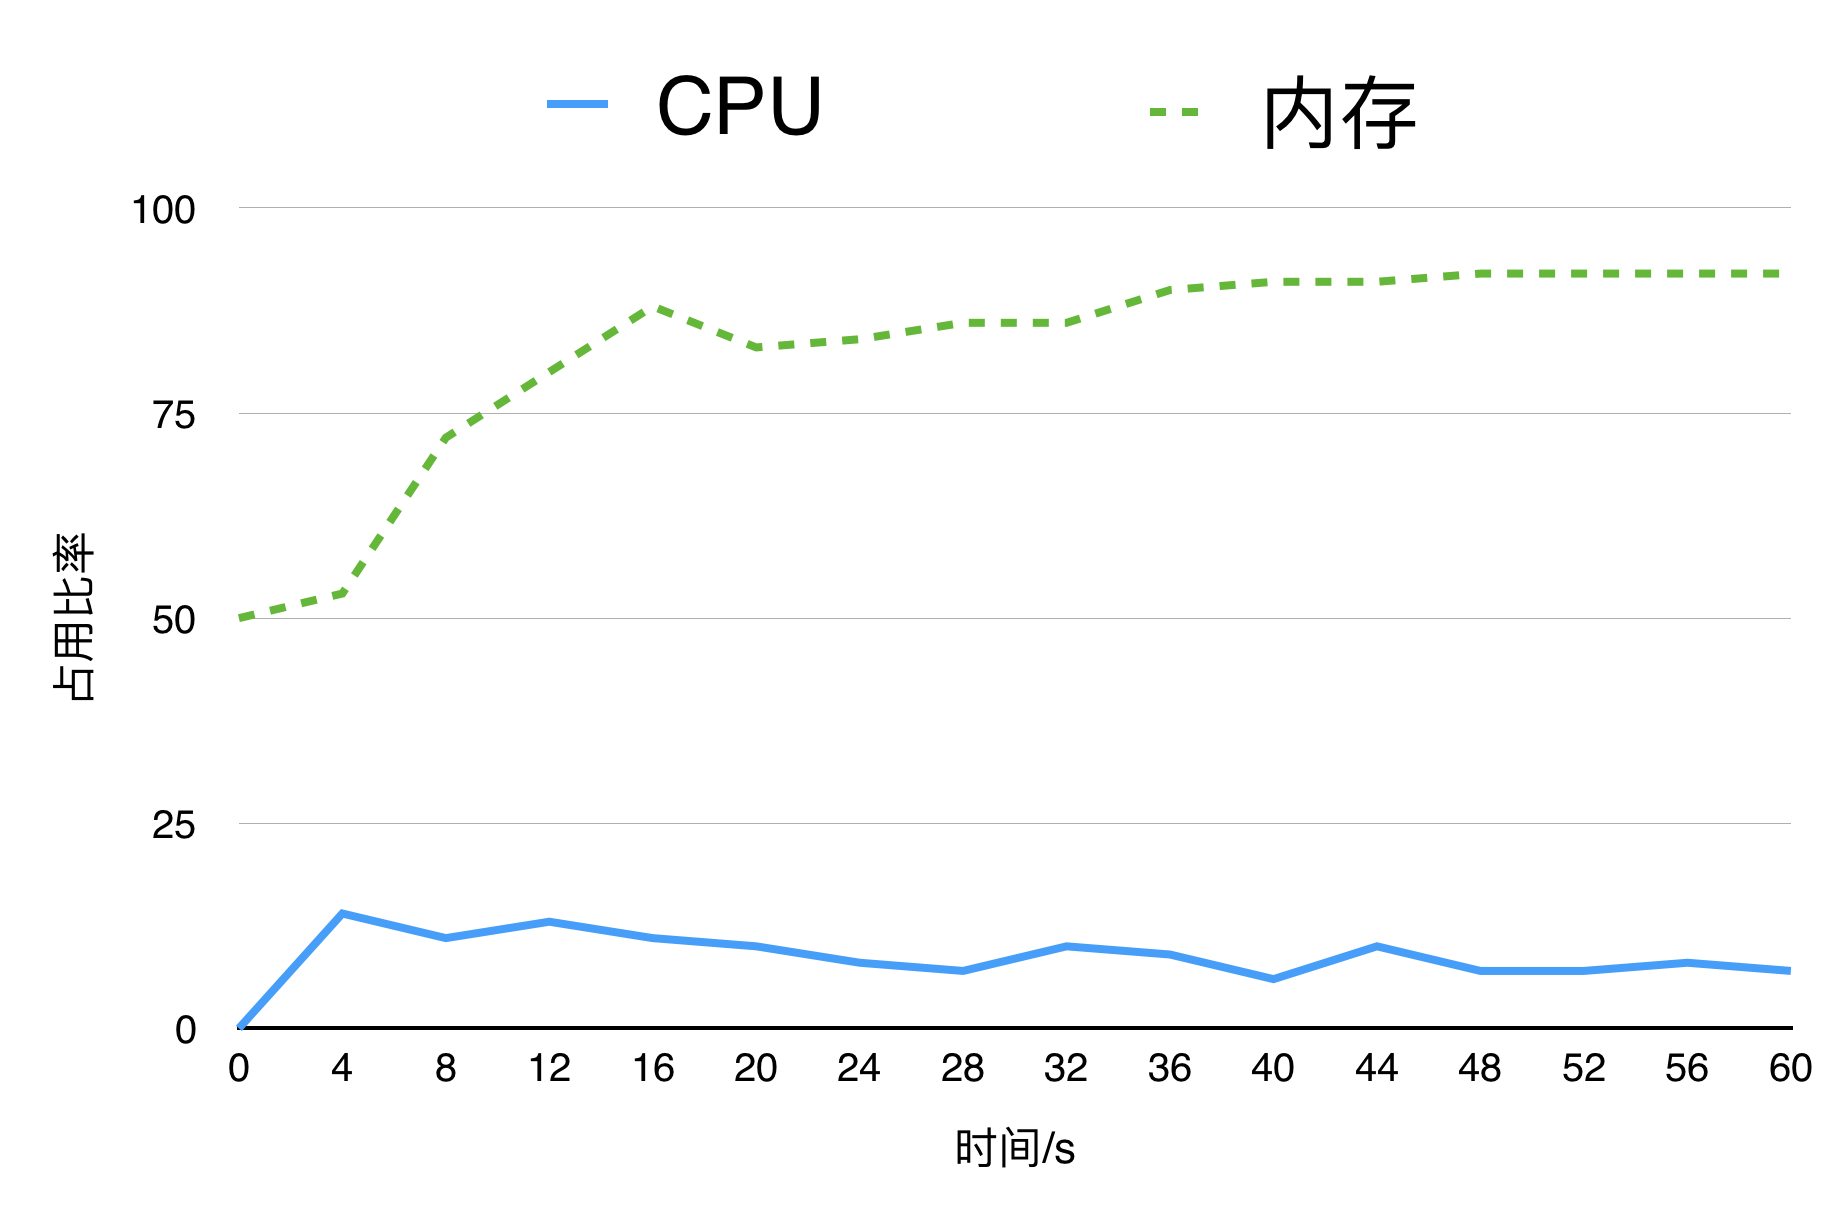
\includegraphics[width=\linewidth]{./graphics/压力测试折线图.png}
	\caption{服务器占用资源变化}
\end{figure}

\newpage